\documentclass[sigplan, anonymous, review]{acmart}

\usepackage{booktabs} % For formal tables


% Copyright
%\setcopyright{none}
%\setcopyright{acmcopyright}
%\setcopyright{acmlicensed}
\setcopyright{rightsretained}
%\setcopyright{usgov}
%\setcopyright{usgovmixed}
%\setcopyright{cagov}
%\setcopyright{cagovmixed}


% DOI
\acmDOI{10.475/123_4}

% ISBN
\acmISBN{123-4567-24-567/08/06}

%Conference
\acmConference[WOODSTOCK'97]{ACM Woodstock conference}{July 1997}{El
  Paso, Texas USA} 
\acmYear{1997}
\copyrightyear{2016}

\acmPrice{15.00}

%\acmBadgeL[http://ctuning.org/ae/ppopp2016.html]{ae-logo}
\acmBadgeR[http://ctuning.org/ae/ppopp2016.html]{ae-logo}


\begin{document}
\title{SIG Proceedings Paper in LaTeX Format}
\titlenote{Produces the permission block, and
  copyright information}
\subtitle{Extended Abstract}
\subtitlenote{The full version of the author's guide is available as
  \texttt{acmart.pdf} document}

\author{Ben Trovato}
\authornote{Dr.~Trovato insisted his name be first.}
\orcid{1234-5678-9012}
\affiliation{%
  \institution{Institute for Clarity in Documentation}
  \streetaddress{P.O. Box 1212}
  \city{Dublin} 
  \state{Ohio} 
  \postcode{43017-6221}
}
\email{trovato@corporation.com}

\author{G.K.M. Tobin}
\authornote{The secretary disavows any knowledge of this author's actions.}
\affiliation{%
  \institution{Institute for Clarity in Documentation}
  \streetaddress{P.O. Box 1212}
  \city{Dublin} 
  \state{Ohio} 
  \postcode{43017-6221}
}
\email{webmaster@marysville-ohio.com}

\author{Lars Th{\o}rv{\"a}ld}
\authornote{This author is the
  one who did all the really hard work.}
\affiliation{%
  \institution{The Th{\o}rv{\"a}ld Group}
  \streetaddress{1 Th{\o}rv{\"a}ld Circle}
  \city{Hekla} 
  \country{Iceland}}
\email{larst@affiliation.org}

\author{Lawrence P. Leipuner}
\affiliation{
  \institution{Brookhaven Laboratories}
  \streetaddress{P.O. Box 5000}}
\email{lleipuner@researchlabs.org}

\author{Sean Fogarty}
\affiliation{%
  \institution{NASA Ames Research Center}
  \city{Moffett Field}
  \state{California} 
  \postcode{94035}}
\email{fogartys@amesres.org}

\author{Charles Palmer}
\affiliation{%
  \institution{Palmer Research Laboratories}
  \streetaddress{8600 Datapoint Drive}
  \city{San Antonio}
  \state{Texas} 
  \postcode{78229}}
\email{cpalmer@prl.com}

\author{John Smith}
\affiliation{\institution{The Th{\o}rv{\"a}ld Group}}
\email{jsmith@affiliation.org}

\author{Julius P.~Kumquat}
\affiliation{\institution{The Kumquat Consortium}}
\email{jpkumquat@consortium.net}


% The default list of authors is too long for headers}
\renewcommand{\shortauthors}{B. Trovato et al.}


\begin{abstract}
This paper provides a sample of a \LaTeX\ document which conforms,
somewhat loosely, to the formatting guidelines for
ACM SIG Proceedings. 
\end{abstract}

%
% The code below should be generated by the tool at
% http://dl.acm.org/ccs.cfm
% Please copy and paste the code instead of the example below. 
%
\begin{CCSXML}
<ccs2012>
 <concept>
  <concept_id>10010520.10010553.10010562</concept_id>
  <concept_desc>Computer systems organization~Embedded systems</concept_desc>
  <concept_significance>500</concept_significance>
 </concept>
 <concept>
  <concept_id>10010520.10010575.10010755</concept_id>
  <concept_desc>Computer systems organization~Redundancy</concept_desc>
  <concept_significance>300</concept_significance>
 </concept>
 <concept>
  <concept_id>10010520.10010553.10010554</concept_id>
  <concept_desc>Computer systems organization~Robotics</concept_desc>
  <concept_significance>100</concept_significance>
 </concept>
 <concept>
  <concept_id>10003033.10003083.10003095</concept_id>
  <concept_desc>Networks~Network reliability</concept_desc>
  <concept_significance>100</concept_significance>
 </concept>
</ccs2012>  
\end{CCSXML}

\ccsdesc[500]{Computer systems organization~Embedded systems}
\ccsdesc[300]{Computer systems organization~Redundancy}
\ccsdesc{Computer systems organization~Robotics}
\ccsdesc[100]{Networks~Network reliability}


\keywords{ACM proceedings, \LaTeX, text tagging}

\begin{teaserfigure}
  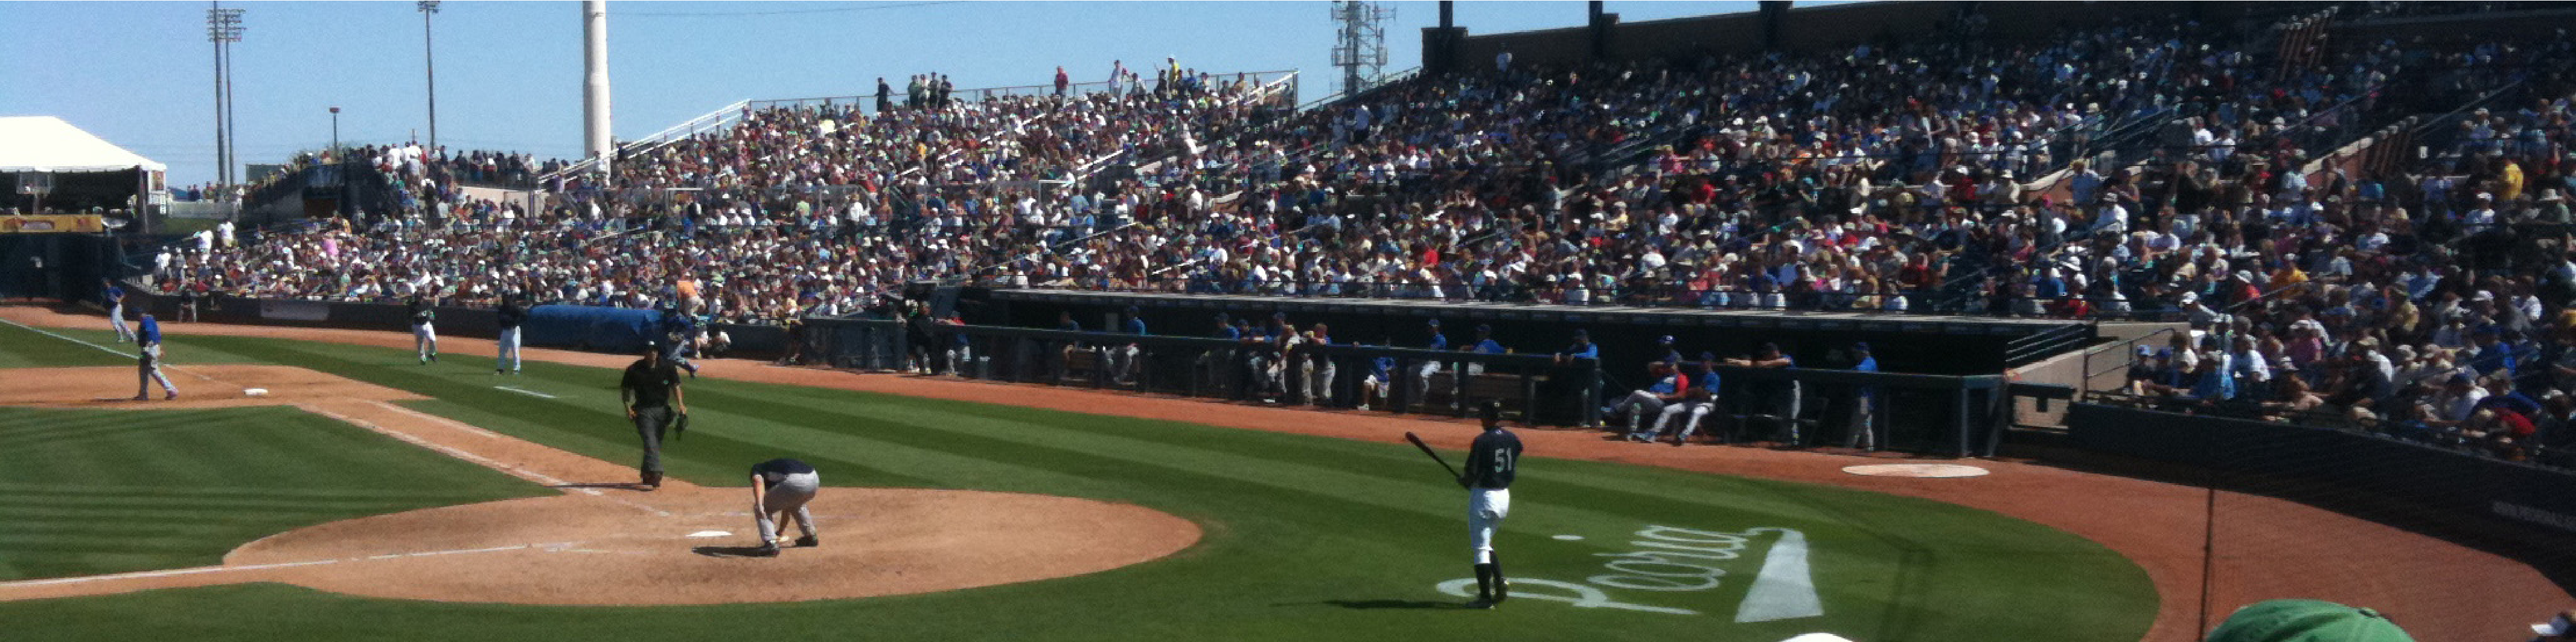
\includegraphics[width=\textwidth]{sampleteaser}
  \caption{This is a teaser}
  \label{fig:teaser}
\end{teaserfigure}


\maketitle

\section{Introduction}

There are tremendous amount of user-generated contents about medical information through the internet. As a result, there is a growing need for enriching medical-related knowledge, for which it can be very valuable for several tasks, such as medical document retrieval, medical question answering, and health-related text mining applications. However, understanding those various health-related contents, especially from social media, is simply not a trivial task since they are written in free text format (i.e. unstructured format), and often prone to grammatical and typographical glitches. Therefore, reducing the complex characteristics of the textual contents, including but not limited to linguistic variations, into structured information could be very beneficial for the text interpretation process. 

One possible solution is to extract medical terms that represents the document they belong to. The common approach is harnessing medical entity recognizer. However, we argue that there are many missing pieces of information when we merely rely on medical entities or terminologies as our main information for representing a particular document. In this paper, we present new keyphrases extraction techniques to extract more important information about the concept expressed inside the document. Furthermore, we also propose a new definition of keyphrases, which is based on our observation of health-related documents. Actually, our final goal is to develop medical question answering systems to assist physicians or people obtaining health information. The work presented in this paper is absolutely inline with our goal, since important keyphrases of a question document can be used to formulate a query for the passage retrieval subsystem. 

Keyphrases are usually selected phrases or clauses that can capture the main topic of a given document \cite{turney2000learning}. They can provide readers with highly valuable and representative information, such that looking at keyphrases is sufficient to understand the whole body of document. Moreover, keyphrases are important for text summarization, document clustering, and classification task (\cite{classDocumentEkp1}; \cite{qaEkp}; \cite{gong2009improving}). Previous works have shown that using keyphrases to generate queries can improve the quality of question retrieval in medical question answering forum \cite{cao2010automatically}.


Keyphrase extraction methods have been mostly using statistical approach (\cite{sparck1972statistical} \cite{zhang2007comparative} \cite{rake} \cite{mihalcea2004textrank}) and supervised learning approach (\cite{witten1999kea} \cite{medelyan2009human} \cite{marujoMAUI}). The statistical approach often involves keyword candidate selection and candidate's property calculation. The "keywordness" value of a candidate phrase is usually scored based on its typical length as well as frequency in which document it appears \cite{rake}. While the statistical approach is very efficient to generate keyphrases, our experiments showed that it performs poorly on user generated contents and short documents. The other approach is based on supervised learning, there are two common approach in supervised learning: classification and sequence labeling. In classification approach, candidate keyphrases are extracted using statistical \cite{sparck1972statistical} or language model \cite{ekpNeuralNetworks}. Then, the candidate keyphrases are classified whether a candidate is a keyphrase or not by using a pretrained model. However, classification approach cannot capture semantic relationship between words in a document \cite{surveyPopulerTerbaruEkp}.  In sequence labeling approach,  like the one proposed by \cite{cao2010automatically} and \cite{zhang2008automatic}. They define keyphrase extraction task as a sequence labeling task, in which each word in the document can have two possible labels: keyword or non-keyword. The method they proposed worked well by outperforming unsupervised approach. However, synonym and ambiguity words cannot be handled properly \cite{zhang2008automatic}.

In our work, we use the same approach as \cite{cao2010automatically} which treats keyphrase extraction as a sequence labeling task. In our experiment, we employed and combined various deep learning architectures, such as convolutional neural networks and bi-directional long short-term memory networks, to exploit high level features between neighboring word positions. To improve the quality of our model, we leverage several new hand-crafted features that can handle our keyphrase extraction problems in medical user-generated content, such as word importance and word stickiness features. The word importance feature is enable to rank words in a document by their importance value. The more important a word is to the content of document, the higher its "keywordness" value would seem to be. In addition, we also propose word stickiness feature to make our model constructs keyphrases better. 

We also employed pre-trained word embedding to incorporate contextual, semantic, and syntactic information of a word. For example, we found that pre-trained word embedding can handle slang words and abbreviations by giving their word vectors closer to the vectors of their canonical forms. Finally, to evaluate the effectiveness of our model, we collected and manually annotated data from Indonesian medical forum questions, such as alodokter, health detik, doktergratis, dokter.id, doktersehat, klikdokter \footnote{www.alodokter.com, health.detik.com, www.dokter.id, www.doktersehat.com, www.klikdokter.com}. After that, the dataset was used for both training and testing our computational models. For our baseline, we use RAKE  \cite{rake}, which is the current state of the art model for extracting keyphrases.


This paper is organized as follows.  In section 2 we discuss related works in keyphrase extraction. In section 3, the proposed keyphrase extraction method has been discussed. We present the evaluation and the experimental results in section 4. 

\section{Related Works}
In general, keyphrase extraction methods can be divided into two groups: unsupervised ranking (statistical) approach and supervised machine learning approach. For the unsupervised line of research, keyphrase extraction is formulated as a ranking problem, in which each candidate keyphrase is assigned a score that represents its keywordness value. Furthermore, this kind of approach does not require training data, which is often very difficult to obtain. On the other hand, supervised machine learning approach requires training data that contains a collection of documents with their labeled keywords. Using this approach, keyphrase extraction is usually treated as a classification or sequence labeling task in the level of words or phrases. The first step of this approach generates candidate keyphrases from a particular document. Finally, every candidate keyphrase in the document will be classified as either a keyphrase or non-keyphrase. Recently, a well-known supervised approach for keyphrase extraction is based on sequence labeling problem (\cite{zhang2008automatic}\cite{cao2010automatically}\cite{zhang2016keyphrase}). The assumption behind this model is that the decision on whether a particular word serves as a keyword is affected by the information from its neighboring word positions.

In the work of \cite{sparck1972statistical}, they leverage TF-IDF to get the most significant words. Specifically, they utilize term frequency and the inverse of document frequency to rank terms in the document. First, this Rapid Automatic Keywords Extraction \cite{rake} uses stopwords to split a document into several candidate keyphrases. All candidates will be ranked by the degrees and frequencies of all words inside them. Finally, the rank points of each candidate is obtained by summing over all degrees and frequencies of all words contained in each keyphrase. RAKE is proven to be successful for extracting keyphrases in special documents such as paper and article \cite{rake}.

There is also a popular graph-based approach, namely TextRank (U), i.e., a modified PageRank algorithm to extract keyphrases from a document. They exploit word co-occurrence information to build a document graph, in which a word serves as a vertice and co-occurence information determines an edge between two vertices (words). After they build the graph, they actually run PageRank algorithm to determine the keywordness score for each vertice in the graph. A word with high PageRank value denotes that its related concept can be found in many location inside the document, which means that it is a good candidate for keyword. After that, keyphrases can be obtained using post-processing step that may combine contiguous candidates into one keyphrase.

One of the earlier supervised approaches in the problem of keyphrase extraction is KEA \cite{witten1999kea}. KEA uses tf-idf and first occurrence of the term to identify candidate keyphrases. They use a machine-learning algorithm (i.e., Naive Bayes) to predict whether or not a candidate is a good keyphrase. \cite{medelyan2009human} developed a system called MAUI that can extract keyphrases using trained corpus and controlled vocabulary. MAUI itself is an improvement to the aforementioned supervised model, KEA. Furthermore, \cite{marujoMAUI} use word embedding and brown clustering as features. Their experiment result had shown that the proposed features and MAUI performs better than statistical methods, such as simple tf-idf approach.

The utilization of neural networks is also quite popular in the recent years. \cite{ekpNeuralNetworks} uses Feed Forward Neural Networks to classify candidate keyphrases. To extract candidate keyphrases, they use POS tag information for classifying all words in the document. Then, Deterministic Finite Automation (DFA) is used to extract noun phrases as candidate keyphrases. Furthermore, deep neural networks is also employed for extracting keyphrase, like the one proposed by \cite{zhang2016keyphrase}, that uses joint Recurrent Neural Networks (RNNs) layer to capture keyphrase sequences in microblogs. The research had shown that RNN is very effective to extract keyword.

Unfortunately, there are limited works regarding the task of keyphrase extraction in medical domain. \cite{ekpMedicalDocumentHybrid} use a hybrid medical knowledge base and statistical approach to extract keyphrases from medical articles. They use stopwords to split candidate keyphrases, then candidates are ranked with two aspects: PF-IDF (Phrase Frequency * Inverse Document Frequency) and domain knowledge which is extracted from medical article. In terms of medical social media content, \cite{cao2010automatically} use Conditional Random Fields (CRFs) for extracting keywords from medical questions in online health-forum. They use information, such as word location and length as features in their experiments.

\section{METHODOLOGY}
\subsection{DATA AND ANNOTATION}
To analyze the effectiveness of our model for keyphrase extraction in user-generated medical domain, we constructed an evaluation dataset. A a number of questions was gathered from Indonesian medical question answering forum. The data was crawled by \cite{skripsiKakRadit} and \cite{skripsiWahid} in their experiment. Generally, we gathered 416 question-answer pairs from \cite{skripsiKakRadit} and \cite{skripsiWahid}. We decided to use the same question-answers pairs to observe our keyphrases and medical entities that has been annotated by them. In addition, system for recognizing medical entities is not fully build, by using the same document we can use the annotated medical entities as our feature.

From analyzing these question-answer pairs, we found some noise and unnecessary information. Question and answer have different main topic and focus. Moreover, we are focusing our task for getting user intentions and needs in our experiment. Based on that problem, we only use questions by users and remove answers by the doctors because it would be a better representation of user intentions and needs. There is also unnecessary information such as URL and email. We replace URL with "URL"  and email with "email" since we were focusing on textual content. Moreover, we also removed ads and spam in the data we gathered.

Because we want to process all the questions by users, we tokenize every question in our data. The tokenization process included separating alphanumeric with non-alphanumeric. Then separating alphanumeric with numeric. 

To evaluate the quality of our model. We manually annotated or data to label keyphrases in 416 questions. In this work, we use "IOB" tagging scheme to label every word \cite{collobert2011natural}. In Table X, we give an example sequence with labels for each word. The statistical information of the dataset can be seen in Table X
\begin{table}
	\caption{Statistical information of dataset. W, K, $\bar{N}_{w}$, $\bar{N}_{k}$ are the total of words, number of keyphrases, average number of words, and average number of keyphrases in each question, respectively.}
	\label{tab:descriptive_stats}
	\begin{tabular}{lcccc}
		\toprule
		\#questions&W&K&$\bar{N}_{w}$&$\bar{N}_{k}$\\
		\midrule
		416 & 26747  & 64.76 & 1861 & 4.49 \\
		
		\bottomrule
	\end{tabular}
\end{table}
\subsection{TASK DEFINITIONS}

\subsection{FEATURES}
Because the small dataset that we have, our model would have a small learning material and an end-to-end approach might not work well. As a result, We leveraged nine handcrafted features that help the model in learning.
\subsubsection{Word embedding\\}
In the experiments, we use word embedding as input to the neural network. A skip-gram model \cite{mikolov2013wordembed} was used to generate these 128-dimensional vectors for documents in evaluation data. The dimension of the vector were chosen based on \cite{skripsiWahid} experiment. The word embeddings we used in this work were trained using a document that we gathered from Indonesia online forum, medical article, and medical question answering forum. 

\subsubsection{Medical Dictionary\\}
In our experiment, we leveraged a medical knowledge base feature using a medical dictionary. Our medical dictionary contains a list of symptom, disease, treatment, and drug in the Indonesian language. The rationale behind this feature is intentions and needs of patients is more focused on their disease, symptom, treatment, and drug. Based on this feature, we classified words by their appearance in the medical dictionary. The dictionary was built by combining three dictionaries from \cite{skripsiKakAbid} research. The original dictionaries contained disease, symptom, treatment, and drug separately in each dictionary.

\subsubsection{Word Length\\}
This feature represents the length of each word (i.e., the number of characters in every word). This feature is based on \cite{cao2010automatically} research on keyphrase extraction in medical question who added word length as a feature because domain-specific words (e.g. "tuberculosis") tend to be lengthy when compared to common English words, and there is a correlation between the length of a word and its IDF value \citep{cao2010automatically}. Thus we use the same feature for Indonesian language.

\subsubsection{Word Position\\}
We also adapted word position as feature based on \cite{cao2010automatically}research. Based on their observation, an important term sometimes appears toward the end of a clinical question. For example, "medicine for bell’s palsy" appear towards the end of question "what is the best medicine for bell’s palsy?". 

\subsubsection{POS-tag\\}
POS-tag of words was also added as our feature. POS-tag may give model grammatical information and a better understanding of ambiguous words. By our observation, many keyphrases have a common POS pattern. For example, "treatment\_Noun for\_Preposition cancer\_Noun", "therapy\_Noun for\_Preposition headache\_Noun". Moreover, \cite{skripsiWahid}, and \cite{abacha2011medical} have proven that POS tag feature has a positive contribution in sequence labeling task in Indonesian medical domain such as Medical Entities Recognizer (MER).

\subsubsection{Medical Entity\\}
We use medical entity which annotated by \cite{skripsiWahid}. By our observation, medical entities are sometimes part of keyphrases. Furthermore, medical entities can provide more information about drug or disease which not available in training data or a medical dictionary.

\subsubsection{Abbreviation and Acronym\\}
We also identified words by their appearance in abbreviation or acronym dictionary gathered by \cite{skripsiKakAbid}. We observed that important word may not be shortened by the users, such as "cancer", "flu", "bell’s palsy".

\subsubsection{Word Importance\\}
We also leveraged a word importance feature. The purpose of this feature is to rank words in a document by their importance. The "keywordness" value of a word can be determined by the importance value. To extract this feature, we adapted a method from TextRank \cite{mihalcea2004textrank} algorithm for ranking words in a document. They represent words as vertices in graph and the distance between words as edges. However, in building an undirected graph, we use a word similarity by using our trained word embedding model. Two words have a connected edge, if their similarity is not negative. The weight of the edge is the similarity itself. Moreover, we use a modified PageRank \cite{page1999pagerank} algorithm that consider edges weight in the calculation. Formally, let $G = (V, E)$ be an undirected graph with the set of vertices V and set of edges E, where E is a subset of $VxV$. For a given vertex $V_i$ let $In(V_i)$ be the set of vertices that point to it (predecessors), and let $Out(V_i)$ be the set of vertices that vertex $V_i$ points to (successors). The modified PageRank formula that proposed by \cite{mihalcea2004textrank} can be seen in Formula \ref{eq:pagerank}.
\begin{equation}\label{eq:pagerank}
	WS(V_{i})=(1-d) + d * \sum_{V_{i} \in In(V_{i})} \frac{w_{ji}}{\sum_{V_{i} \in Out(V_{j})}}w_{jk}
\end{equation}

\subsubsection{Word Stickiness\\}
As a keyphrase, a sequence must be in a valid order. There is some noise such as misuse punctuation by users. For example, "Saya mengalami pusing pada jidat sakit perut dan pandangan kabur (I am having a headache on forehead stomachache and blurred vision)", there is no comma between "jidat (forehead)", "sakit perut (stomachache)" and "dan (and)". Our model may mistake the sequence "(jidat sakit perut)forehead stomachache" as a keyphrase. Based on that problem, we propose a feature that may capture how likely of a given word is occurred together with the word before and after. We use Pointwise Mutual Information (PMI) of a bigram probability to capture the likeness. This feature represented as two dimensional vector $v = [x1, x2]$, with $x_1$ is the PMI with the word before and $x_2$ is the PMI with the word after. Formula \ref{eq:pmi} is the formula for calculating the PMI value. In that formula, $p(x)$ is the occurrence probability of word $x$, $p(y)$ is the occurrence probability of word $y$, and $p(x, y)$ is the probability of word $x$ and $y$ co-occur together.
\begin{equation}\label{eq:pmi}
	PMI(x,y)=log(\frac{p(x, y)}{p(x)*p(y)})
\end{equation} 
\subsection{MODEL ARCHITECTURE}
We process the sequences word by word. Features are extracted from every word as the input representation of the model. The output for this words are label which describe a word is either part of keyphrase or not.

To give our model a better insight of context, we introduce Convolutional Neural Networks (CNNs) to capture context from three adjacent words.  From our observation, to know whether a word is part of keyphrase or not, we need to know the context of the word itself. For example, "Doc, i have a frequent back pain. What happen?". The keyphrase for previous example is "frequent back pain". In order to know that "back" is part of keyphrase, we need information from the word "frequent" which give an intensity of a symptom and "pain" which refer to "back pain" as main term. With CNNs, we argue that our model can capture the surrounding information of a word.

To get a better inference, information from the past and future sequences can be integrated. This approach is proven effective  in sequence labeling task such as semantic role labeling \cite{SMRzhou2015end} and named entity recognition \cite{ma2016end}. Hence, we utilized  bi-directional LSTM (B-LSTM) for extracting structural knowledge by processing sequences both forward and backward. We build up to two layers of B-LSTM.
To perform the sequence tagging task, we build a fully connected layer in the top of our model. This layer will classify the output of our model with softmax activation function.

We also experimented on customizing the way we input the features underneath our aforementioned networks. Instead of concatenating all feature into one vector, we tried to give weight for every feature we have. We argue that each feature have different contribution to the model. In order to do so, we create a new layer underneath our model to do the weighting scenario. The following equation to weight all feature can be seen in below:
\begin{equation}
Z =  tanh(W _{1}*F_{1} + W_{2}*F_{2} + .. + W_{n}*F_{n})
\end{equation}
Where $W_{i}$ are the weight for each feature and $F_{i}$ are the extracted feature in vector form.
\section{EXPERIMENTS}
In this section, we analyzed the importance of our features by conducting a feature ablation study. Furthermore, we also established a scenario to test the performance of our model.
\subsection{Evaluation}
One of the evaluation that we use in our work is using partial evaluation. This evaluation is used because we treat keyphrases as sequences of words. Thus we can use partial evaluation which is used to evaluate Named Entity Recognition system. In partial evaluation method, a assigned keyphrase is predicted correctly if a predicted keyphrase has a word which is a subset in assigned keyphrase words. 

We use Recall, Precision, and F1 score as our evaluation parameters. Recall shows the number of correctly predicted keyphrases divided by the the total number of assigned keyphrases and Precision is the number of correctly predicted keyphrase divided by the total number of predicted keyphrases. To calculate F1 score we use Recall and Precision as parameters which is 2  Recall  Precision/ (Recall + Precision).
\subsection{Feature Ablation Study}
In this part, perform a feature ablation study. By considering all the features, and then removing one of these features, we want to estimate the importance of the features. To the experiment. We use 80\% as training set, and 20\% as a testing set. We used precision (P), recall (R), and F1-score (F1) as evaluation metrics. Table \ref{tab:ablation} show the experimental result. Then, we use LSTM as evaluation model because it is the most simple architecture. These are the following features we proposed: word stickiness (Ws), word abbreviation and acronym (Wa), Medical Entities (Me), Word Location (Wp), Word Length (Wl), Word Importance (Wi), POS tag (Pt), Medical Dictionary (Md).

\begin{table*}
	\caption{Feature Ablation Study Result}
	\label{tab:ablation}
	\begin{tabular}{lccc}
		\toprule
		Features&Precision&Recall&F-Measure\\
		\midrule
		We + Ws + Wa + Me + Wp + Wl + Wi + Pt + Md & \textbf{84.01\%} & 75.79\% & \textbf{79.69\%} \\
		
		Ws + Wa + Me + Wp + Wl + Wi + Pt + Md & 79.93\% & 57.45\% & 66.85\% \\
		
		We + Wa + Me + Wp + Wl + Wi + Pt + Md & 76.39\% & 73.59\% & 74.96\% \\
		
		We + Ws + Me + Wp + Wl + Wi + Pt + Md & 78.44\% & 73.83\% & 76.07\% \\
		
		We + Ws + Wa + Wp + Wl + Wi + Pt + Md & 79.38\% & 76.28\% & 77.8\% \\
		
		We + Ws + Wa + Me + Wl + Wi + Pt + Md & 74.24\% & \textbf{78.23\%} & 76.19\% \\
		
		We + Ws + Wa + Me + Wp + Wi + Pt + Md & 75.36\% & 76.28\% & 75.82\% \\
		
		We + Ws + Wa + Me + Wp + Wl + Pt + Md & 83.69\% & 75.3\% & 79.27\% \\
		
		We + Ws + Wa + Me + Wp + Wl + Wi + Md & 79.68\% & 74.81\% & 77.17\% \\
		
		We + Ws + Wa + Me + Wp + Wl + Wi + Pt & 75.66\% & 76.03\% & 75.85\% \\
		\bottomrule
	\end{tabular}
\end{table*}


The experimental results in Table \ref{tab:ablation} shows that every feature has a positive contribution to the model. It is shown by iteratively remove each feature one by one and every time we remove a feature, F-1 score always dropped. Hence, we use every feature to train our model in the next experiments.
\subsection{Model Scenario}
We created a scenario to evaluate the performance of our model. In this scenario, we also compared our model to an unsupervised learning algorithm using RAKE. Moreover, we also implemented CRF to as a baseline for this sequence labeling task. CRF also has been proven effective in extracting keyphrases \cite{cao2010automatically} \cite{zhang2008automatic}. The following scenarios are listed below:
\begin{itemize}
	\item RAKE
	\item CRF
	\item B-LSTM
	\item CNN-B-LSTM
	\item Weighting-CNN-B-LSTM
\end{itemize}
The result of the scenario can be seen in Table \ref{tab:model_scenario}.
\begin{table}
	\caption{Model Scenario Result}
	\label{tab:model_scenario}
	\begin{tabular}{lccc}
		\toprule
		Models&Precision&Recall&F-Measure\\
		\midrule
		RAKE & 43.24\% & 68.19\% & 52.90\% \\
		
		CRF & 63.44\% & 64.94\% & 62.52\% \\
		
		LSTM & 78.77\% & 79.71\% & 79.16\% \\
		
		B-LSTM & 81.88\% & \textbf{83.05\%} & 82.37\% \\
		
		CNN-B-LSTM & \textbf{82.00\%} & 82.99\% & \textbf{82.41\%} \\
		
		\bottomrule
	\end{tabular}
\end{table}
Table \ref{tab:model_scenario} shows the performance of different methods that we proposed on dataset we have. To evaluate or model we use 10-cross fold validation. From the results, we observed that every supervised method using sequence labeling approach achieved a better performance than RAKE. The best result achieved by CNN with two stacked B-LSTM with 82.41\% F-Score. RAKE Perform the worst. The result shows that RAKE only achieved 52.9\% F-Score. This is because RAKE using statistical approach to weight candidate keyphrases which becoe a problem in short document like medical questions. Furthermore, RAKE using stopwords to split candidate keyphrases in document, but user-generated content tend to have a bad structural information. Thus there are some misplaced stopwords in the content. Among other methods, CRF performed the worst. Bidirectional approach shows effectiveness because B-LSTM has a better result than LSTM. Furthermore, using CNN to capture context between words also shows improvement and it become the best result in our experiment. However, when we use CRF on the top of our model the results dropped. The experiment results indicated our context aware CNN and B-LSTM worked well in keyphrase extraction in Indonesian user-generated medical domain. 

We also tried our feature weighting layer in our best model which is CNN with B-LSTM and fully-connected hidden layer on top. The result in Table \ref{tab:weighting_scenario} shows that our weighting layer not worked quite well. We suspect the gap of information between features are on of the reason which cause the result drop
\begin{table}
	\caption{Weighting Layer Scenario Result}
	\label{tab:weighting_scenario}
	\begin{tabular}{lccc}
		\toprule
		Models&Precision&Recall&F-Measure\\
		\midrule
		CNN-B-LSTM & 82.00\% & 82.99\% & 82.41\% \\
		
		W-CNN-B-LSTM & 81.08\% & 81.18\% & 81.01\% \\
		\bottomrule
	\end{tabular}
\end{table}
\subsection{Error Analysis}
We performed an error analysis to the aforementioned model, the result shown there are several errors. Some of the error are uncompleted keyphrases. For example "headache on (sakit kepala pada)", "medicine for (obat untuk)". Our model also failed to capture complex medicine name and disease. This is due to our small data set and not all medicine and disease are captured in our knowledge base. Moreover, there are also special case for keyphrases like "treatment for headache and sore throat (penyembuhan untuk sakit kepala dan tenggorokan)", that keyphrase need to be captured as whole because "sore throat" have a connection with the word "treatment". But our model, failed to capture that connection, it extracted "treatment for headache" and "sore throat" separately.
\section{Conclusion}
We investigate a keyphrase extraction problem especially in Indonesian medical questions domain with sequence labeling approach. We leverage a deep learning approach using CNN and B-LSTM. Moreover, we also extracted nine features that capture medical concepts from a knowledge base, and linguistic components as our features. With this model and features, we are able to overcome problems such as informal language, short document, and medical domain specific. Our model achieves F1 score of 82.41\% on manually annotated Indonesian medical questions.

For handling several problems that occurred in this experiment, we suggest to create a language model for post-processing. The language model expected to handle cases like uncompleted keyphrase or connection between keyphrase.

Furthermore, we realized that there are no solid evaluation method for keyphrase extraction. Partial evaluation may handle how the model extract sequences in a document. However, weights for importance in sequences are different between words. For example "therapy for pregnancy", in that keyphrase we may realize that "pregnancy" is more important than other words. Thus partial evaluation failed to capture that problem.


\bibliographystyle{ACM-Reference-Format}
\bibliography{sigproc} 

\end{document}
